% !Mode:: "TeX:UTF-8"%确保文档utf-8编码
%commands:
%environments:  
\documentclass[xetex,compress]{mybeamer}
%8pt, 9pt, 10pt, 11pt, 12pt, 14pt, 17pt, 20pt
%draft – no graphics, footlines,...
%handout – no overlays
%xcolor=x11names – define more names for colors
%,aspectratio=169


\usetheme{Singapore}
\usecolortheme{rose}
%albatross fly crane seagull beetle wolverine dove beaver
% innercolortheme lily orchid rose               the colors of blocks. 
%outer color theme whale seahorse dolphin          headline, footline, and sidebar




\title{改性Bi{\scriptsize 2}O{\scriptsize 3}基光催化剂的制备\\[10pt]及其光催化性能研究}
%\subtitle
%\date
%\institute
%\logo
\author{答辩人:万泽}
\institute{指导教师:××× 教授}
\logo{
\includegraphics[scale=0.2]{figures/四川理工学院图标.jpg}}
\date{2013年12月19日}

\begin{document}

\begin{frame}
\titlepage
\end{frame}
%plain  for large firgure  , fragile   can catcode ,mainly for verbatim environment


\begin{frame}
\frametitle{目录}
\setcounter{tocdepth}{1}
\tableofcontents[pausesections]%pausesections section pause
\end{frame}


\section{前言}%beamer class divided into section subsection subsubsection
%section* etc add to navigation bars not the toc
\subsection{引言}
\begin{frame}
\frametitle{引言}
\begin{block}{}
太阳能是唯一可再生的碳中性能源,取之不尽用之不竭,是化石能源的良好替代品。直接利用太阳能作为清洁能源是二十一世纪科学界的重大挑战。尤其在目前能源短缺和环境污染问题日益严重的背景下,不管是直接利用太阳能分解水制备氢气还是直接利用太阳能参与某些化学反应等都具有非常重要的意义。
\end{block}
\end{frame}


\subsection{光催化机理}
\begin{frame}
\frametitle{光催化机理}
\begin{columns}
\column{0.5\textwidth}
\begin{block}{}
\centering
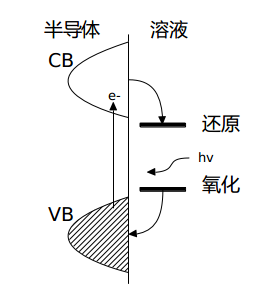
\includegraphics[scale=0.6]{figures/光催化机理图} 
\end{block}
\column{0.5\textwidth}
\begin{block}{}
半导体有一个禁带能宽,当照射进来的光的能量超过禁带能宽时,就会把价带(VB)的电子激发并进入导带(CB)。这样在价带会形成空穴,而在导带会形成额外的电子,通常这些空穴—电子对是成对出现的。
\end{block}
\end{columns}
\end{frame}



\begin{frame}
\frametitle{Fujishima的开创性工作}
\begin{block}{}
\centering
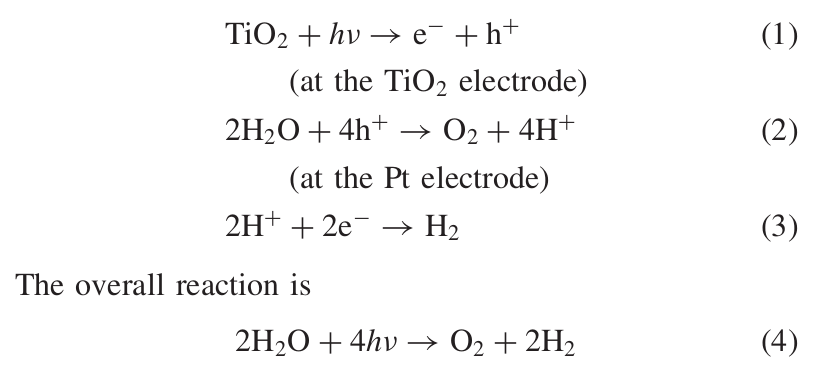
\includegraphics[scale=0.3]{figures/光分解水化学反应式} 
\end{block}
\begin{block}{}
其中TiO2是光电阳极释放电子,Pt是光电阴极在这里释放氧气。整个反应就是水的分解反应。这个光化学电池量子效率是非常低下的,大约为0.1。
\end{block}
\end{frame}

\subsection{纳米三氧化二铋的性质}
\begin{frame}
\frametitle{纳米三氧化二铋的性质}
\begin{columns}
\column{0.7\textwidth}
\begin{block}{}
\centering
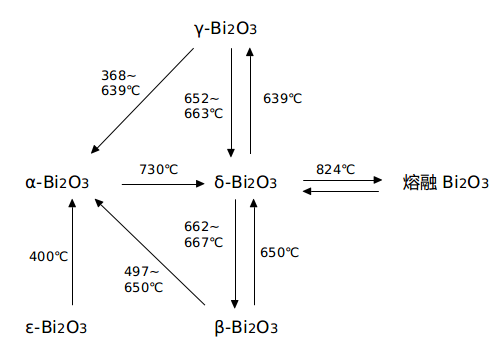
\includegraphics[width=\linewidth]{figures/Bi2O3转变温度} 
\end{block}
\column{0.3\textwidth}
\begin{block}{}
其中α-Bi2O3是室温下最稳定的构型,α-Bi2O3的禁带能宽为2.85 eV,对大部分可见光都应有吸收和响应。
\end{block}
\end{columns}
\end{frame}

\begin{frame}
\frametitle{三氧化二铋的缺陷}
\begin{columns}
\column{0.5\textwidth}
\begin{block}{光生电子—空穴复合率过高}
其中光生电子—空穴对复合率过高主要是通过调整光催化材料的晶体结构,比如通过提高结晶度加速光生电子—空穴对的分离,或者更细小的纳米粒子也会促进光生电子和空穴的分离。
\end{block}
\column{0.5\textwidth}
\begin{block}{结构不太稳定}
而Bi2O3结构不太稳定的问题Lei Huang做了专门的探讨。α-Bi2O3在空气中存放6个月就会部分转变成Bi2O2CO3,这一过程在水溶液中会进一步加速进行,这可能是因为空气中的CO2溶于水生成HCO3-和α-Bi2O3发生了反应。
\end{block}
\end{columns}
\end{frame}

%<1>  first show <2> second show [<+->]依次显示 <1-2>1,2都显示 <1->从1一直显示

















\end{document}
